\section{Checking Balance}
\label{sec:balance}

\subsection{Quick Overview}

To check balance, use \texttt{summary(m.out)} for numerical summaries
and \texttt{plot(m.out)} for graphical summaries.

\subsection{Details}

\subsubsection{The {\tt summary()} Command}

The \texttt{summary()} command gives measures of the balance between
the treated and control groups in the full (original) data set, and
then in the matched data set.  If the matching worked well, the
measures of balance should be smaller in the matched data set (smaller
values of the measures indicate better balance).

The \texttt{summary()} output for subclassification is the same as
that for other types of matching, except that the balance statistics
are shown separately for each subclass, and the overall balance in the
matched samples is calculated by aggregating across the subclasses,
where each subclass is weighted by the number of units in the
subclass.  For exact matching, the covariate values within each
subclass are guaranteed to be the same, and so the measures of balance
are not output for exact matching; only the sample sizes in each
subclass are shown.

\begin{itemize}
\item {\bf Balance statistics:} The statistics the \texttt{summary()}
  command provides include means, the original control group standard deviation (where applicable), 
  mean differences, standardized mean
  differences, and (median, mean and maximum) Quantile-Quantile (Q-Q)
  plot differences.  In addition, the \texttt{summary()} command will
  report (a) the matched call, (b) how many units were matched,
  unmatched, or discarded due to the \texttt{discard} option
  (described below), and (c) the percent improvement in balance for
  each of the balance measures, defined as $100((|a|-|b|)/|a|)$, where
  $a$ is the balance before and $b$ is the balance after matching.
  For each set of units (original and matched data sets, with weights
  used as appropriate in the matched data sets), the
  following statistics are provided:
\begin{enumerate}
  \item ``Means Treated'' and ``Means Control'' show the weighted
    means in the treated and control groups
  \item ``SD Control" is the standard deviation calculated in the control group (where applicable)
  \item ``Mean Diff'' is the difference in means between the groups
  \item The final three columns of the summary output give summary
    statistics of a Q-Q plot (see below for more information on these
    plots). Those columns give the median, mean, and maximum distance
    between the two empirical quantile functions (treated and control
    groups).  Values greater than 0 indicate deviations between the
    groups in some part of the empirical distributions.  The plots of
    the two empirical quantile functions themselves, described below,
    can provide further insight into which part of the covariate
    distribution has differences between the two groups.
\end{enumerate}

\item {\bf Additional options:} Three options to the \texttt{summary()}
  command can also help with assessing balance and respecifying the
  propensity score model, as necessary.  First, the {\tt interactions
    = TRUE} option with {\tt summary()} shows the balance of all
  squares and interactions of the covariates used in the matching
  procedure.  Large differences in higher order interactions usually
  are a good indication that the propensity score model (the distance measure) needs to be
  respecified.  Similarly, the {\tt addlvariables} option with {\tt
    summary()} will provide balance measures on additional variables
  not included in the original matching procedure.  If a variable (or
  interaction of variables) not included in the original propensity score model
  has large imbalances in the matched groups, including that
  variable in the next model specification may improve the resulting
  balance on that variable.  Because the outcome variable is not used
  in the matching procedure, a variety of matching methods can be
  tried, and the one that leads to the best resulting balance chosen.  Finally,
  the {\tt standardize = TRUE} option will print out standardized versions of the
  balance measures, where the mean difference is standardized (divided) by the standard deviation
  in the original treated group.
\end{itemize}

\subsubsection{The \texttt{plot()} Command}

We can also examine the balance graphically using the \texttt{plot()}
command, which provides three types of plots: jitter plots of the
distance measure, Q-Q plots of each covariate, and histograms of the
distance measure.  For subclassification, separate Q-Q plots can be
printed for each subclass.  The jitter plot for subclassification is
the same as that for other types of matching, with the addition of
vertical lines indicating the subclass cut-points.  With the histogram
option, 4 histograms are provided: the original treated and control
groups and the matched treated and control groups.  For the Q-Q plots
and the histograms, the weights that result after matching are used to
create the plots.

Three examples of the output from the {\tt plot()} command are shown
in Figure~\ref{fig:plotcommandoutput}.  If the empirical distributions
are the same in the treated and control groups, the points in the Q-Q
plots would all lie on the 45 degree line (lower left panel of
Figure~\ref{fig:plotcommandoutput}).  Deviations from the 45 degree
line indicate differences in the empirical distribution.  The jitter
plot (top panel) shows the overall distribution of propensity scores
in the treated and control groups.  In the jitter plot, which can be
created by setting \texttt{type = "jitter"}, the size of each point is
proportional to the weight given to that unit.  Observation names can
be interactively identified by clicking the first mouse button near
the units.  The histograms (lower right panel) can be plotted by
setting \texttt{type = "hist"}.

\begin{figure}
  \begin{center}
  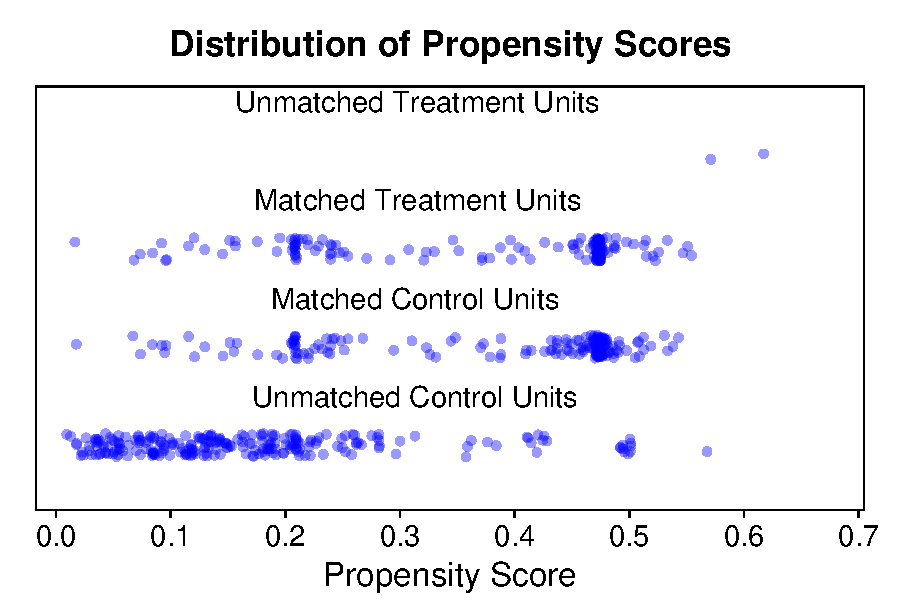
\includegraphics[height=2.7in, keepaspectratio=true]{figs/jitterplotnn.pdf}
  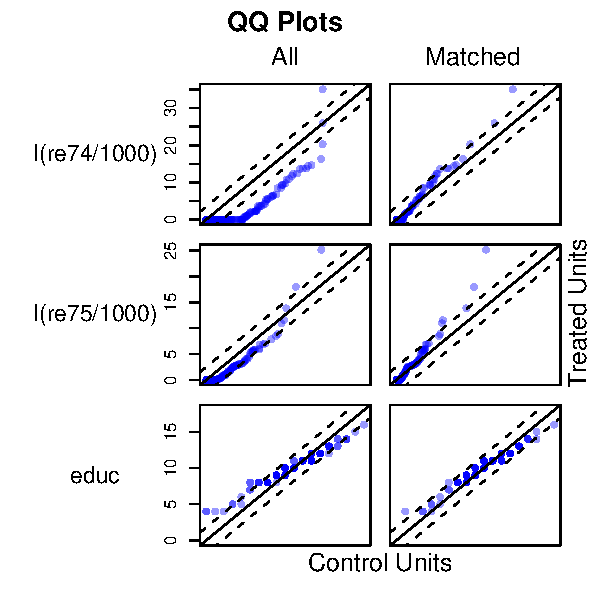
\includegraphics[height=3in,keepaspectratio=true]{figs/qqplotnn1.pdf}
  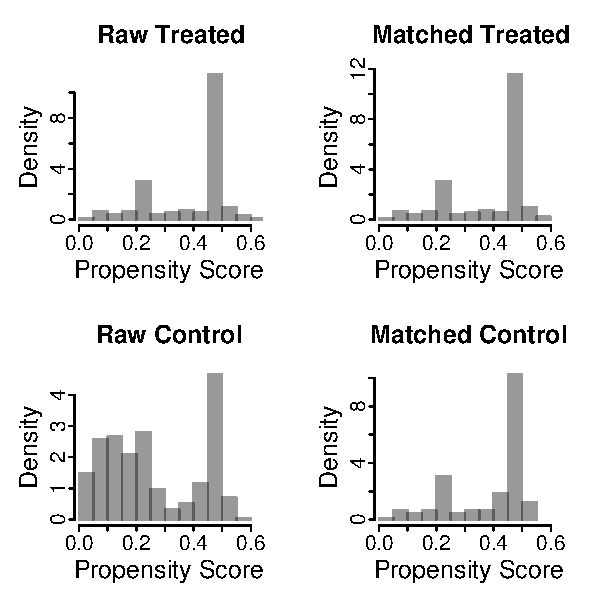
\includegraphics[height=3in,keepaspectratio=true]{figs/hist.pdf}
  \caption{Examples of the three types of output from the
    \texttt{plot} command resulting from matching on the
    /texttt{lalonde} data set based on real earnings in 1974
    (\texttt{re74}) divided by 1000, real earnings in 1975
    (\texttt{re75}) divided by 1000, years of education
    (\texttt{educ}), Hispanic (\texttt{hispan}) and marital status
    (\texttt{married}).  Observations in both the treated and the
    control groups outside the support of the distance measure were
    discarded.  The upper plot shows the jitter plot of the distance
    measure.  The lower left plot shows the QQ plots for the first
    three covariates (\texttt{I(re74/1000)}, \texttt{I(re75/1000)},
    \texttt{educ}).  The lower right plot shows the histograms of the
    density of propensity scores for observations before and after
    matching.}
  \label{fig:plotcommandoutput}
\end{center}
\end{figure}


%%% Local Variables: 
%%% mode: latex
%%% TeX-master: "matchit"
%%% End: 
